\begin{figure}
\centering

\newcommand{\myWidth}{0.98\linewidth}
\begin{subfigure}{\myWidth}
    \centering
    \caption{Learning rate $=10^{-3}$}
    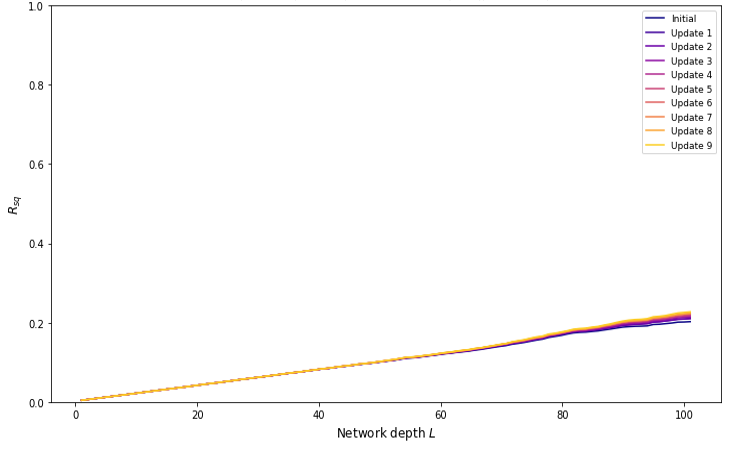
\includegraphics[width=\myWidth]{img/Sec5/sim1/Rsq_for_each_layer_0001(hard-tanh_50ave)}
    \label{fig:sec5sim15_a}
\end{subfigure}
\begin{subfigure}{\myWidth}
    \centering
    \caption{Learning rate $=10^{-2}$}
    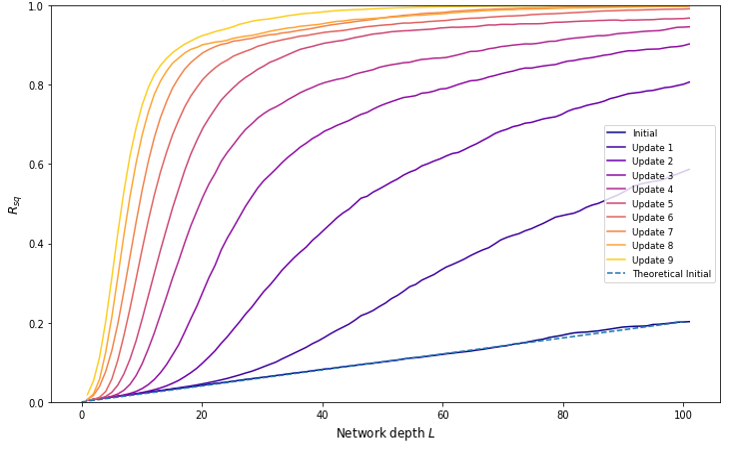
\includegraphics[width=\myWidth]{img/Sec5/sim1/Rsq_for_each_layer(hard-tanh_50ave)}
    \label{fig:sec5sim15_b}
\end{subfigure}
\caption[The dynamics of VNI $R_{sq}$ of hidden layers.]
{
    The dynamics of VNI $R_{sq}$ of hidden layers.
The training is performed on the MNIST dataset 50 times, and then we evaluate the averages of hidden layer
VNI $R_{sq}$ for learning rates $\in\{10^{-3}, 10^{-2}\}$.
%It shows that overall, the correlation of each hidden layer is intensified during the back-propagation training. For large learning rate, the output VNI $R_{sq}$ severely increases to 1.
}
\label{fig:sec5_sim15}
\end{figure}
